\documentclass[11pt]{jsarticle}

\usepackage{SPR}

\headerSPR
\begin{document}
	\titleSPR{\number\year}{\number\month}{\number\day}{D2}{吉田 皓太郎}
%%%%%%%%%%%%%%%%%%%%%%%%%%%%%%%%%%%%%%
	\articleSPRabst
		\begin{itemize}
			\item 機械学習を用いたカップ形状の設計支援
			\item 着後形状予測のためのカップの変形解析
		\end{itemize}
		
		
	\articleSPRobj
		\begin{enumerate}
			\item 定性的な機能要求を満たせるようなカップ形状を設計できる
			\item 布の物性とカップのパターンがどのような結びつきを持っているかを調べることができる.
		\end{enumerate}
%%%%%%%%%%%%%%%%%%%%%%%%%%%%%%%%%%%%%%
% 1.前回からのノルマ
	\articleSPRitemsone
		%\begin{enumerate}
		%	\item A
		%\end{enumerate}
		
		\tableofcontents
		
		
%%%%%%%%%%%%%%%%%%%%%%%%%%%%%%%%%%%%%%
%\begin{itemize}
%	\item 新規手法について
%	\item ISFAアウトライン
%\end{itemize}
%%%%%%%%%%%%%%%%%%%%%%%%%%%%%%%%%%%%%%
% 2.具体的な成果
	\articleSPRitemstwo
	\renewcommand{\labelitemi}{$\blacktriangledown$}
%%%%%%%%%%%%%%%%%%%%%%%%%%%%%%%%%%%%%
	\section{研究進捗について}
		先週の研究成果等について報告いたします.
		\begin{itemize}
			\item 機械学習を用いたシステムの概要について
			\item これからのTodo
		\end{itemize}
		\subsection{機械学習を用いたシステムの概要について}
			\begin{figure}[h!]
				\centering
				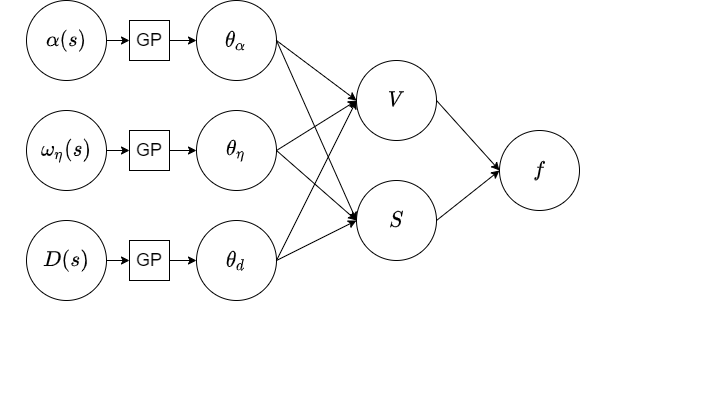
\includegraphics[scale=0.5]{./figure/systems.png}
				\caption{SYSTEM}
			\end{figure}
			機械学習におけるシステムの概要を文字に起こすと,次のようにまとめられます.
			\begin{itemize}
				\item ガウス・ボネの原理より,第一基本量,第二基本量によって可展面の情報は一意に決定される.これらの基本量は次式に示す形によって表されている.したがって,この可展面情報を一意に決定する関数群$ \alpha $,$ \omega_{\eta} , \omega_{\xi}$,$ D $を機械学習によって学習することができればよい.(厳密には$ D $は式中には出てこないが,$ t $の定義域が$ [0,D(s)] $であることから,特徴的であるとしている)
				\begin{eqnarray}
				E &=& (\alpha'+\lambda)^2 t^2 -2\cos \alpha(\alpha'+\lambda) t + 1,\\
				F &=& -\sin \alpha,\\
				G &=& 1,
				\end{eqnarray}
				
				\begin{eqnarray}
				L &=& -\omega_{\xi}+t\{\lambda(-\omega_{\xi}\cos \alpha + \omega_{\zeta}\sin \alpha)+\omega_{\zeta}'\cos \alpha + \omega_{\xi}'\sin \alpha \},  \\
				M &=& \omega_{\xi}\sin \alpha + \omega_{\zeta} \cos \alpha,  \\
				N &=& 0. 
				\end{eqnarray}
				また,先週にも述べたように,$  \omega_{\eta} , \omega_{\xi} $とワイヤーの空間曲率$ \kappa (s) $の間には,以下の関係が存在すること,また,データにおける前提としてワイヤーデータはすべて同じものを使っているということから,$ \omega_{\xi} $は$ \omega_{\eta} $に関して従属的に決定できる.
				\begin{equation}\label{eq:kappaeq}
					\omega_{\eta}^2 + \omega_{\xi}^2 = \kappa^2
				\end{equation}
				このことから,$ \omega_{\xi} $は特徴量から除外でき,可展面を決定するのは関数群$ \alpha $,$ \omega_{\eta} $,$ D $の3つの関数である.
				
				\item 次に問題となるのが,この3つの関数をどのような特徴空間(パラメータ空間)$ S_p $へ,できるだけ$ \dim{S_p} $を小さくしつつ射影するかである.そこで,本研究では,可展面データにおける$ \alpha $,$ \omega_{\eta} $,$ D $を,GPを用いてハイパーパラメータベクトル$ \bd{\theta}_{\alpha},\bd{\theta}_{\eta},\bd{\theta}_{D} $を抽出することで,$ \dim{S_p} $を小さくしつつ,特徴空間へ射影できると考えた.このベクトル$ \bd{\theta} = [\theta_1 \;\; \theta_2 \;\; \theta_3] $の各成分は,次式で示すRBF+Linearカーネル式中に現れるパラメータである.
				
				\begin{equation}\label{eq:RBFLinear}
					k(x_i,x_j) = \theta_1 \exp \left( -\frac{(x_i-x_j)^2}{\theta_2} \right) + \theta_3 x_i x_j
				\end{equation}
				
				\item カップの囲う体積および表面積によって評価関数$ f(V,S) $を計算する.
				
				「囲う」および「押さえる」を決定する要因を,それぞれカップの囲う体積および表面積とバストにおけるそれらとの差分$\Delta V,\Delta S $で表現できるものとする.
				\begin{itemize}
					\item $ |\Delta S| $が小さければ,十分に囲えてることが示されている
					\item $ \Delta V $が小さい(負の方向に大きくなる)場合,押さえる度合が大きいことが示されている
				\end{itemize}
				上記を考慮し,評価関数を以下のように設定する.
				\begin{equation}\label{eq:EvalFunc}
					f(V,S) = \phi_1 \frac{\Delta V}{V_b} \exp \left(-\phi_2 \left(\frac{\Delta S}{S_b}\right)^2 \right)
				\end{equation}
				
				\item 上記を用いて,入力パラメータを$ \bd{\theta}_{\alpha},\bd{\theta}_{\eta},\bd{\theta}_{D} $に対する出力を$ f $とし学習データを作成,$ f(\bd{\theta}_{\alpha},\bd{\theta}_{\eta},\bd{\theta}_{D}) $をGPを用いて回帰予測を行う.
				
				現在,学習データが1100個程度あり,これを
				\begin{itemize}
					\item 学習用データ 900個
					\item 検証用データ 200個
				\end{itemize}
			に分けて,実行したいと思っております.現在,上記のプログラムを実行し,パラメータ化を行っている最中である.
			\end{itemize}
		\subsection{これからのTodo}
			\begin{itemize}
				\item 最後の機械学習もGPを使うと..なんか同じことを繰り返しているだけな気がするので,ディープラーニング等を用いて何か別の回帰予測を行う手法について検討したい.もしくは,GPに一工夫が欲しい.
				\item データを作り直し,二枚接ぎカップ全体で学習用データを作りたい.
			\end{itemize}
			
	\newpage
\vspace{10cm}
%%%%%%%%%%%%%%%%%%%%%%%%%%%%%%%%%%%%%%
% 3.達成できなかったこととその問題点
	%\articleSPRthree
	
%%%%%%%%%%%%%%%%%%%%%%%%%%%%%%%%%%%%%%

\vspace{14cm}
%%%%%%%%%%%%%%%%%%%%%%%%%%%%%%%%%%%%%%
	\articleSPRfour
	\articleSPRfive
\end{document}
